\documentclass[10pt,a4paper]{article}
\usepackage{fontspec,amsmath,amssymb,amsthm,mathtools,graphicx,bm,bbm,stmaryrd}
\usepackage[margin=22mm]{geometry}
\usepackage[bookmarks=false]{hyperref}
\setlength{\emergencystretch}{3em}
\makeatletter
\renewcommand\author[1]{\gdef\@author{\parbox{\textwidth}{\centering #1}}}
\makeatother
\title{Almost independent distributions separated by logarithmic-width DNFs}
\author{Yaroslav Alekseev, Mika Göös, Ziyi Guan, Gilbert Maystre, Artur Riazanov, Dmitry Sokolov, Weiqiang Yuan}
\date{doi:10.4230/LIPIcs.CCC.2025.29; CC BY 4.0}
\begin{document}
\maketitle
\noindent\textit{Editorial note.} Editable TeX faithfully converted from official CC BY HTML prose and math alttext. Full source-local proofs, bibliography and original PDF/HTML retained. Only selected independent main theorem counts; all parameter and model conditions retained.\par\medskip
\noindent\textit{Editorial note.} SVG assembly correction: official HTML object graphics restored at their original paragraph positions. Original SVGs, faithful vector PDF conversions and URL/license ledger are included; all existing author text and captions are retained.\par\medskip
\noindent\textit{Allowed standard prerequisites (editorial).}\begin{itemize}
\item Standard probability, circuits and finite-group representation background. All author local support retained.
\end{itemize}\medskip


\par\medskip\noindent\textbf{
1 Introduction}\par




Linial and Nisan [16] conjectured that “$k$-wise independent” distributions fool constant-depth circuits (class $\textsf{AC}^{0}$). More specifically, a distribution $\mathcal{D}$ over $\{0,1\}^{n}$ is called \emph{$k$-independent} if the marginal distribution on every $k$-sized subset of bits is uniform. We say that $\mathcal{D}$ \emph{$\delta$-fools} a circuit $C$ if the circuit cannot distinguish $\mathcal{D}$ from the uniform distribution on $\{0,1\}^{n}$:\par


\[\begin{gathered}
\Big{|}\Pr_{\bm{x}\sim\mathcal{D}}[C(\bm{x})=1]-\Pr_{\bm{x}\sim\{0,1\}^{n}}[C(\bm{x})=1]\Big{|}\nobreak\ \leq\nobreak\ \delta.
\end{gathered}\]


The Linial–Nisan conjecture was first proved for depth-2 circuits (DNFs and CNFs) by Bazzi [4] (with a simplification by Razborov [21]) and then for every $\textsf{AC}^{0}$-circuit by Braverman [7]. Indeed, Braverman showed that every size-$s$ $\textsf{AC}^{0}$-circuit is $o(1)$-fooled by $\mathrm{poly}(\log s)$-independence.\par




Aaronson [1] asked whether the Linial–Nisan conjecture could be strengthened to hold also for “almost $k$-wise independence,” a seemingly modest generalisation. We say that a distribution $\mathcal{D}$ over $\{0,1\}^{n}$ is \emph{$(\varepsilon,k)$-independent} if for every subset $I\subseteq[n]$, $|I|=k$, the marginal distribution on the bits in $I$ is multiplicatively close to uniform in the sense that for every $\alpha\in\{0,1\}^{I}$,\par


\[\begin{gathered}
(1-\varepsilon)2^{-k}\nobreak\ \leq\nobreak\ \Pr\limits_{\bm{x}\sim\mathcal{D}}[\bm{x}_{I}=\alpha]\nobreak\ \leq\nobreak\ (1+\varepsilon)2^{-k}.
\end{gathered}\]



% SOURCE-ID Thmglnx1


\par\medskip\noindent\textbf{
\textbf{Generalised Linial–Nisan Conjecture (GLN)}\textbf{.}
}\par



\emph{Let $\mathcal{D}$ be a $(1/n^{\Omega(1)},n^{\Omega(1)})$-independent distribution over $\{0,1\}^{n}$. Then $\mathcal{D}$ $o(1)$-fools every $\textsf{AC}^{0}$-circuit of size $2^{n^{o(1)}}$.}\par



% END-SOURCE-ID Thmglnx1



Aaronson’s original motivation for this conjecture was to resolve a problem in quantum complexity theory. He showed that a positive resolution of GLN would imply the separation $\textsf{BQP}\nsubseteq\textsf{PH}$ relative to an oracle. (This separation was subsequently proved by Raz and Tal [20] by a different approach.) Later, Aaronson himself found a counterexample to GLN for depth-3 circuits [2], but he still re-posed the conjecture (and thought it “plausible”) for depth-2 circuits. Our main result here is to refute the GLN conjecture in this remaining case.\par




% SOURCE-ID Thmtheorem1


\par\medskip\noindent\textbf{
\textbf{Theorem 1}\textbf{ }(Main result)\textbf{.}
}\par



\emph{There exists a $(1/n^{\Omega(1)},n^{\Omega(1)})$-independent distribution $\mathcal{D}$ over $\{0,1\}^{n}$ and a $O(\log^{3}n)$-width DNF formula $F$ such that}\par


\[\begin{gathered}
\Pr_{\bm{x}\sim\mathcal{D}}[F(\bm{x})=1]-\Pr_{\bm{x}\sim\{0,1\}^{n}}[F(\bm{x})=1]\nobreak\ \geq\nobreak\ \Omega(1).
\end{gathered}\]



% END-SOURCE-ID Thmtheorem1




Let us make two notes about the parameters here.
First, our formula $F$ will have quasi-polynomial size, whereas Aaronson’s depth-3 counterexample has only polynomial size; hence his example achieves slightly better parameters (at the cost of larger depth). Second, our construction can be varied to produce the following tradeoff: by increasing the DNF width to any $w\leq n^{o(1)}$, we can make the distribution $(\exp(-w^{\Omega(1)}),n^{\Omega(1)})$-independent (see Section 2.5).\par




\par\medskip\noindent\textbf{
1.1 Implications and related work}\par




One consequence of the failure of the GLN conjecture is to the construction of \emph{pseudorandom generators} (PRGs) for DNFs. It is known that for $k\geq\Omega(\log n)$ there exist $(o(1),k)$-independent distributions with support size $2^{O(k)}$ [18, 3], which is smaller than $n^{\Omega(k)}$ that is required for truly $k$-wise independent distributions [8]. Thus Theorem 1 rules out a natural approach (“output an almost $k$-wise independent distribution”) to improving the seed length of PRGs. For the current state-of-the-art PRGs for DNFs, see [9, 22, 17]; see also the survey [13].\par




Another lesson from Theorem 1 is to the further development of circuit lower bound methods. We find it important to seek alternative proofs of central theorems such as Bazzi’s [4, 21] and its extensions [7]. The existing proofs use the \emph{polynomial method} to approximate a DNF with a low-degree polynomial. Is there a more “combinatorial” proof of Bazzi’s theorem? One such more combinatorial approach is the \emph{top-down} lower bound method [12, 11], which often uses entropy-based arguments to analyse circuits. We interpret the failure of GLN as a challenge to such top-down methods. While the method is in a formal sense \emph{complete} (it can prove any lower bound that is true), the typical entropy counting arguments have a hard time distinguishing almost $k$-wise independent distributions from truly $k$-wise independent ones, suggesting that any top-down proof of Bazzi’s theorem would require substantially new ideas.\par




Finally, we mention that – besides (almost) $k$-wise independence – several other notions of pseudorandomness have been considered in the literature [6, 5, 14].\par





\par\medskip\noindent\textbf{
1.2 Workaround: Local couplings}\par




To complement our main result, we also propose a way to circumvent the failure of GLN by proposing a new notion of pseudorandomness called \emph{local couplings}. This notion is useful for fooling depth-2 circuit models, but not depth-3 models; in particular, we show the following claims:\par


\begin{enumerate}


\item[] 
1. 


Local couplings fool DNFs (query complexity analogue of NP).\par





\item[] 
2. 


Local couplings fool decision lists (query complexity analogue of $\textsf{P}^{\textsf{NP}}$).\par





\item[] 
3. 


Local couplings do \emph{not} fool depth-3 circuits (query complexity analogue of $\Sigma_{2}\textsf{P}$).\par





\end{enumerate}



% SOURCE-ID Thmtheorem2


\par\medskip\noindent\textbf{
\textbf{Definition 2}\textbf{ }(Local couplings)\textbf{.}
}\par



\emph{A pair of jointly distributed random variables $(\bm{x},\bm{y})\in(\{0,1\}^{n})^{2}$ is an $\varepsilon$-semi-coupling if for every $y\in\mathrm{supp}(\bm{y})$ and $i\in[n]$,}\par


\[\begin{gathered}
\Pr[\bm{x}_{i}\neq\bm{y}_{i}\mid\bm{y}=y]\leq\varepsilon.
\end{gathered}\]


\emph{We say that $(\bm{x},\bm{y})$ is an
$\varepsilon$-coupling if both $(\bm{x},\bm{y})$ and $(\bm{y},\bm{x})$ are $\varepsilon$-semi-couplings.}\par



% END-SOURCE-ID Thmtheorem2



The notion of a local coupling was somewhat implicit in Aaronson’s analysis [2] of his depth-3 counterexample. Local couplings are also a stronger variant of a notion proposed by Zhandry [23] that he called “substitution distance.”\par




\par\medskip\noindent\textbf{Claims 1–2
}\par




A width-$k$ \emph{decision list} is a sequence of pairs $\{(T_{i},a_{i})\}_{i\in[m]}$ where $T_{i}$ are $k$-terms (conjunctions of at most $k$ literals) and $a_{i}\in\{0,1\}$ are output values. A decision list defines $f\colon\{0,1\}^{n}\to\{0,1\}$ as follows: $f(x)=a_{i}$ where $i=\min\{i\in[m]\mid T_{i}(x)=1\}$. The decision list width of a function is polynomially equivalent to the number of $\mathrm{DNF}$ queries necessary to compute the function [10, Appendix A]. In other words it is indeed a query complexity analogue of $\textsf{P}^{\textsf{NP}}$. The following theorem (Section 3.1) formalises 1–2 when $\bm{y}$ is uniformly distributed.\par



% SOURCE-ID Thmtheorem3


\par\medskip\noindent\textbf{
\textbf{Theorem 3}\textbf{.}
}\par



\emph{Let $f$ be computed by a width-$k$ decision list. For any $\varepsilon$-coupling $(\bm{x},\bm{y})$,}\par


\[\begin{gathered}
\Pr[f(\bm{x})\neq f(\bm{y})]\leq 2k\varepsilon.
\end{gathered}\]



% END-SOURCE-ID Thmtheorem3




\par\medskip\noindent\textbf{Claim 3
}\par




Aaronson’s [2] original counterexample involved a distribution $\mathcal{D}$ related to a certain \emph{surjectivity} function, which can be computed by a small depth-3 circuit. We observe (Section 3.2) that Aaronson’s distribution $\mathcal{D}$ can indeed be locally coupled with the uniform distribution, which implies that local couplings do not fool depth-3 circuits (Claim 3). We can furthermore conclude (using Theorem 3) that $\mathcal{D}$ fools decision lists – this claim was already made earlier by Aaronson [2, Theorem 3], but his proof contained a mistake,\footnote{The mistake is acknowledged on the author’s homepage. An implication of this result would have been to show the separation $\Pi_{2}\textsf{P}\neq\textsf{P}^{\textsf{NP}}$ relative to a random oracle. That result however follows (using a function different from surjectivity) from the more recent result that PH is infinite in the random oracle model [15].} which we can now fix with the notion of local couplings. Finally, we also show (Section 3.3) that an $\varepsilon$-semi-coupling is not enough by itself to fool DNFs – one truly needs the two-sided condition of an $\varepsilon$-coupling.\par







\par\medskip\noindent\textbf{
2 Counterexample}\par




In this section, we prove Theorem 1 by constructing a DNF formula $F$ and an associated almost $k$-independent distribution $\mathcal{D}$ that $F$ can distinguish from uniform. We first (Section 2.1) construct a weak example that distinguishes $\mathcal{D}$ from uniform with advantage $1/\mathrm{poly}(\log n)$. Then (Section 2.4) we amplify this advantage to $\Omega(1)$ by using a standard majority trick.\par




\par\medskip\noindent\textbf{
2.1 Construction}\par




Our starting point is the \emph{address} function $\textsc{Addr}\colon\{0,1\}^{m}\times\{0,1\}^{2^{m}}\to\{0,1\}$ defined as $\textsc{Addr}(a,p):=p_{a}$. Here we write $p_{a}$ to mean $p_{\text{int}(a)}$ where $\text{int}(a)\in[2^{m}]$ is the integer corresponding naturally to the bitstring $a$. Let us first observe that Addr together with the uniform distribution over $\textsc{Addr}^{-1}(1)$ “almost works” as the counterexample in Theorem 1. For $(\bm{a},\bm{p})\sim\textsc{Addr}^{-1}(1)$ the distribution of $\bm{p}$ is already $(o(1),2^{\Omega(m)})$-independent. The reason the whole $(\bm{a},\bm{p})$ does not have the same property is that for example, fixing all bits of $\bm{a}$ to some $a$ forces $\bm{p}_{a}=1$, so for some $I\subseteq[m+2^{m}]$ containing all bits describing $\bm{a}$ and the bit $\bm{p}_{a}$ the settings of $(\bm{a},\bm{p})_{I}$ with $\bm{p}_{a}=0$ have probability zero.\par




To avoid this issue we hide the bits of the address using the usual \emph{tribes} function:\par


\[\begin{gathered}
\textsc{Tribes}(A):=\bigvee_{j\in[r]}\bigwedge_{k\in[m]}A_{k,j}.
\end{gathered}\]


The input here is an $m\times r$ boolean matrix and the function returns $1$ iff the matrix contains an all-$1$ column. It is well-known [19, §4.2] that if we choose $r:=\lceil 2^{m}\ln 2\rceil$, the function becomes \emph{balanced}, meaning that $\Pr_{\bm{A}\sim\{0,1\}^{m\times r}}[\textsc{Tribes}(\bm{A})]=1/2+o(1)$.\par




A natural attempt to define a counterexample would be to consider the distinguishing function $\textsc{Addr}((\textsc{Tribes}(A^{1}),\dots,\textsc{Tribes}(A^{m})),p)$. This does not work since this function requires polynomial $\mathrm{DNF}$ width as the negation of Tribes reduces to it. We fix this by replacing the Addr function by its \emph{monotone} version: $\textsc{mAddr}\colon\{0,1\}^{m}\times\{0,1\}^{2^{m}}\to\{0,1\}$ is defined as\par


\[\begin{gathered}
\textsc{mAddr}(a,p):=\begin{cases}0&\quad\text{if $|a|<m/2$}\\
p_{a}&\quad\text{if $|a|=m/2$}\\
1&\quad\text{if $|a|>m/2$}\end{cases},\quad\text{ where $|a|$ is the Hamming weight of $a$.}
\end{gathered}\]


We are now ready to define our function
$f\colon(\{0,1\}^{m\times r})^{m}\times\{0,1\}^{2^{m}}\to\{0,1\}$ by (see also Figure 1)\par


\[\begin{gathered}
f(A^{1},\dots,A^{m},p):=\textsc{mAddr}((\textsc{Tribes}(A^{1}),\dots,\textsc{Tribes}(A^{m})),p),
\end{gathered}\]


Note that input size of $f$ is $n:=m^{2}r+2^{m}$. The following constructs a narrow DNF for $f$.\par
\par\noindent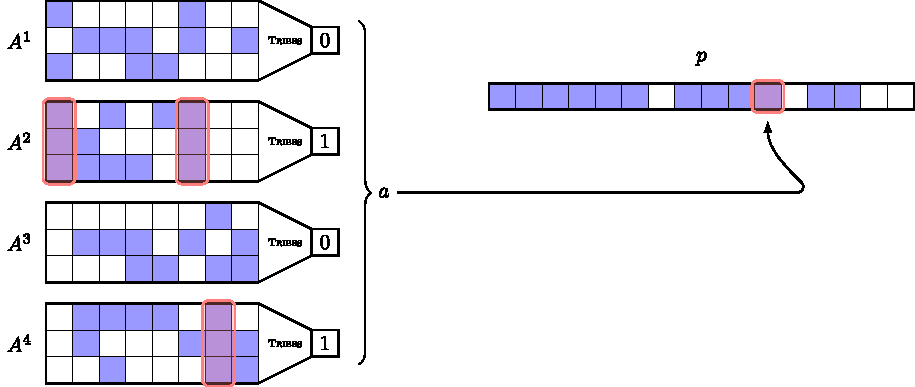
\includegraphics[width=\linewidth,height=0.78\textheight,keepaspectratio]{ccc2025-29-svg-01.pdf}\par



Figure 1: Illustration of $\textsc{mAddr}(\textsc{Tribes}(A^{1}),\dots,\textsc{Tribes}(A^{4}),p)$. Blue cells correspond to $1$-input bits, white cells correspond to $0$-input bits. The
address $a=(\textsc{Tribes}(A^{1}),\dots,\textsc{Tribes}(A^{4}))$ is $(0,1,0,1)$, so it satisfies $|a|=4/2$. Hence the function outputs $p_{\text{int}(a)}=p_{11}=1$.


% SOURCE-ID Thmtheorem4


\par\medskip\noindent\textbf{
Claim 4. 
}\par



There exists a $\mathrm{DNF}$ $F$ of width $O(\log^{2}n)$ that computes $f$.\par



% END-SOURCE-ID Thmtheorem4



\par\medskip\noindent\textbf{
\textbf{Proof}.}\par




A $\mathrm{DNF}$ is commonly viewed as a collection of \emph{$1$-certificates}: $f$ is computable by a $k$-$\mathrm{DNF}$ iff for each point $x\in f^{-1}(1)$ there exists a certificate comprised of a subset of input bits $I\subseteq[n]$ of size $k$ and $\alpha\in\{0,1\}^{I}$ such that $x^{\prime}_{I}=\alpha$ implies $f(x^{\prime})=1$. Hence it is enough to provide a certificate of width $O(m^{2})=O(\log^{2}n)$ for each $1$-input of $f$. Consider a $1$-input $x=(A^{1},\dots,A^{m},p)$ and let $a:=(\textsc{Tribes}(A^{1}),\dots,\textsc{Tribes}(A^{m}))$. If $|a|>m/2$, a $1$-certificate is simply a set of matrices $H\subseteq[m]$ of size $|H|=m/2+1$ together with a $1^{m}$-column in each of those matrices. Such certificates fix $(m/2+1)\cdot m$ variables. A similar idea can certify $1$-inputs with $|a|=m/2$, at the cost of adding the corresponding bit $p_{a}$.
$\vartriangleleft$\par




We now define $\mathcal{D}$ as a distribution of the random variable $\bm{x}$ defined below.\par



% SOURCE-ID Thmtheorem5


\par\medskip\noindent\textbf{
\textbf{Definition 5}\textbf{.}
}\par



\emph{Let $\bm{x}=(\bm{A}^{1},\bm{A}^{2},\dots,\bm{A}^{m},\bm{p})$ over $\{0,1\}^{n}$ be sampled as follows:}\par


\begin{enumerate}


\item[] 
1. 


\emph{Sample }$\bm{A}^{i}\sim\{0,1\}^{m\times r}$\emph{ uniformly and independently for each }$i\in[m]$\emph{.}\par





\item[] 
2. 


\emph{Sample }$\bm{p}\sim\{0,1\}^{2^{m}}$\emph{ uniformly and independently.}\par





\item[] 
3. 


\emph{Let }$\bm{a}=\big{(}\textsc{Tribes}(\bm{A}^{1}),\dots,\textsc{Tribes}(\bm{A}^{m})\big{)}$\emph{; If }$|\bm{a}|=m/2$\emph{,
fix }$\bm{p}_{\bm{a}}=1$\emph{.}\par





\end{enumerate}



% END-SOURCE-ID Thmtheorem5



We show that $\mathcal{D}$ is $(n^{-1/5},n^{1/5})$-independent, yet $f$ distinguishes $\mathcal{D}$ from the uniform
distribution, which together with Claim 4 implies the following weaker version
of Theorem 1:\par



% SOURCE-ID Thmtheorem6


\par\medskip\noindent\textbf{
\textbf{Lemma 6}\textbf{.}
}\par



\emph{The distribution $\mathcal{D}$ as in Definition 5 is $(n^{-1/5},n^{1/5})$-independent, but there is
an $O(\log^{2}n)$-$\mathrm{DNF}$ $F$ such that
$\Pr_{\bm{x}\sim\mathcal{D}}[F(\bm{x})=1]-\Pr_{\bm{x}\sim\{0,1\}^{n}}[F(\bm{x})=1]=\Omega(\log^{-1/2}n).$}\par



% END-SOURCE-ID Thmtheorem6



We reduce the proof of Lemma 6 to the following two lemmas:\par



% SOURCE-ID Thmtheorem7


\par\medskip\noindent\textbf{
\textbf{Lemma 7}\textbf{.}
}\par



$\Pr_{\bm{x}\sim\mathcal{D}}[f(\bm{x})=1]-\Pr_{\bm{x}\sim\{0,1\}^{n}}[f(\bm{x})=1]=\Omega\big{(}1/\sqrt{m}\big{)},$\emph{
where $m$ is as in Definition 5.}\par



% END-SOURCE-ID Thmtheorem7


% SOURCE-ID Thmtheorem8


\par\medskip\noindent\textbf{
\textbf{Lemma 8}\textbf{.}
}\par



\emph{The distribution $\mathcal{D}$ as in Definition 5 is $(\varepsilon,k)$-independent for $k\leq 2^{m}$, $\varepsilon\leq k2^{-m/2+1}$.}\par



% END-SOURCE-ID Thmtheorem8




\par\medskip\noindent\textbf{Proof of Lemma 6.}\par




$\mathcal{D}$ is distributed over $\{0,1\}^{n}$ where $n:=m^{2}\lceil 2^{m}\ln 2\rceil+2^{m}$. Apply Lemma 8 with $k=n^{1/5}$ and $\varepsilon=n^{1/5}2^{-m/2+1}\ll n^{-1/5}$. Then by Lemma 7 and Claim 4 there exists $O(m^{2})=O(\log^{2}n)$-$\mathrm{DNF}$ that $\Omega(1/\sqrt{m})=\Omega(1/\sqrt{\log n})$-distinguishes $\mathcal{D}$ from $\mathcal{U}$, where the latter is uniformly distributed over $\{0,1\}^{n}$.
$\blacktriangleleft$\par






\par\medskip\noindent\textbf{
2.2 Proof of Lemma 7
}\par




Let $\bm{x}:=(\bm{A}^{1},\dots,\bm{A}^{m},\bm{p})\sim\mathcal{D}$ and $\bm{y}\sim\{0,1\}^{n}$. Since the matrices $\bm{A}^{i}$ are uniformly generated, it is possible to couple $\bm{x}$ and $\bm{y}$ by defining $\bm{y}:=(\bm{A}^{1},\dots,\bm{A}^{m},\bm{p}^{\prime})$ where $\bm{p}^{\prime}\sim\{0,1\}^{2^{m}}$. Note that the address part of each input coincides and in particular, they share the event $E:=\text{``$|\bm{a}|=m/2$''}$.\par




Observe that $\Pr[f(\bm{x})=1\mid\lnot E]=\Pr[f(\bm{y})=1\mid\lnot E]$ by the definition of $\mathcal{D}$: if $|\bm{a}|\neq m/2$ then Step (3) is not reached in the definition of $\mathcal{D}$ and $\bm{p}$ is uniform. On the other hand we have $\Pr[F(\bm{x})=1\mid E]=1$. Indeed, if $E$ holds, we have $F(\bm{x})=\bm{p}_{\bm{a}}=1$ by the definition of $f$ and $\mathcal{D}$.\par


\[\begin{gathered}
\displaystyle\Pr[F(\bm{y})=1\mid E] \displaystyle=\Pr[\bm{p}^{\prime}_{\bm{a}}=1\mid E] \\
\displaystyle=\sum_{a\in\{0,1\}^{m}}\Pr[\bm{p}^{\prime}_{a}=1\mid E\land\bm{a}=a]\Pr[\bm{a}=a\mid E] \\
\displaystyle=\sum_{a\in\{0,1\}^{m}}\Pr[\bm{p}^{\prime}_{a}=1]\Pr[\bm{a}=a\mid
E]=\frac{1}{2}.
\end{gathered}\]


Thus, $\Pr[f(\bm{x})=1]-\Pr[f(\bm{y})=1]=\Pr[E]/2$ and so it remains to bound $\Pr[E]$. For that, we need the following simple fact:\par



% SOURCE-ID Thmtheorem9


\par\medskip\noindent\textbf{
\textbf{Lemma 9}\textbf{.}
}\par



\emph{Let $\bm{x}$ distributed over $\{0,1\}^{n}$ according to a product distribution such that
$|\Pr[\bm{x}_{i}=1]-1/2|\leq\varepsilon$. Then $\Delta(\bm{x},\bm{u}):=\max_{E\subseteq\{0,1\}^{n}}\big{|}\Pr[\bm{x}\in E]-\Pr[\bm{u}\in E]\big{|}\leq 2n\varepsilon$, where $\bm{u}\sim\{0,1\}^{n}$.}\par



% END-SOURCE-ID Thmtheorem9



\par\medskip\noindent\textbf{Proof.}\par




Let us couple $\bm{x}$ with $\bm{u}$ as follows:
suppose $\Pr[\bm{x}_{i}=1]=1/2+p$. We then set $\bm{u}_{i}:=\bm{x}_{i}$ with
probability $1/(1+2|p|)$ and $\bm{u}_{i}:=\llbracket p>0\rrbracket:=(1\text{ if }p>0\text{ otherwise }0)$
with probability $1-1/(1+2|p|)\leq 2|p|\leq 2\varepsilon$.
Then $\Pr[\bm{U}_{i}=1]=(1/2+p)/(1+2|p|)+\llbracket p>0\rrbracket(1-1/(1+2|p|))=1/2$, so $\bm{u}$ is indeed uniformly distributed.
Then $\Pr[\bm{x}\neq\bm{u}]\leq 2n\varepsilon$, so $\Delta(\bm{x},\bm{u})\leq 2n\varepsilon$.
$\blacktriangleleft$\par




Note that each bit $\bm{a}_{i}$ is close to being balanced:\par


\[\begin{gathered}
\Pr[\bm{a}_{i}=1]=1-(1-2^{-m})^{r}=1-(1/e+\Theta(2^{-m}))^{\ln 2}=1/2+\Theta(2^{-m}).
\end{gathered}\]


As all $\bm{a}_{i}$ are independent, we can use Lemma 9 to get sharp bounds on their sum being exactly $m/2$: $\Pr[E]\geq\Pr_{\bm{x}\sim\{0,1\}^{m}}[|\bm{x}|=m/2]-\Theta(m\cdot 2^{-m})=\Omega(1/\sqrt{m})$.\par






\par\medskip\noindent\textbf{
2.3 Proof of Lemma 8
}\par




We need to show that for every $I\subseteq[n]$ of size $k$ and for every $\alpha\in\{0,1\}^{I}$ we
have $(1-\varepsilon)\cdot 2^{-k}\leq\Pr[\bm{x}_{I}=\alpha]\leq(1+\varepsilon)\cdot 2^{-k}$. We
now classify the bits of $I$ and $\alpha$. Let $I_{i}\subseteq[m]\times[r]$ for $i\in[m]$ be the set
of bits of $\bm{A}^{i}$ in $I$. Let $J\subseteq\{0,1\}^{m}$ be the set of bit indices of $\bm{p}$ that
belong to $I$ (we identify the indices with their bit representations). Let $\alpha^{i}\in\{0,1\}^{I_{i}}$
and $\beta\in\{0,1\}^{J}$ be the corresponding parts of $\alpha$.\par




Since $\bm{A}^{1},\dots,\bm{A}^{m}$ are uniformly distributed it suffices to show that\par


\[\begin{gathered}
(1-\varepsilon)2^{-|J|}\leq\Pr[\bm{p}_{J}=\beta\mid\forall i\in[m]:\bm{A}^{i}_{I_{i}}=\alpha^{i}]\leq(1+\varepsilon)2^{-|J|}.
\end{gathered}\]


Let
$J^{m/2}:=\{s\in J\mid|s|=m/2\}.$
Intuitively the only non-uniformity in $\bm{x}_{I}$ is introduced when $\bm{a}\in J^{m/2}$ as this is the
only case where $\bm{p}$ is changed from uniform. We make this intuition precise in the following claim.\par



% SOURCE-ID Thmtheorem10


\par\medskip\noindent\textbf{
Claim 10. 
}\par



For any event $E$ that is a function of $\bm{A}^{1},\ldots,\bm{A}^{m}$ we have\par


\[\begin{gathered}
(1-\Pr[\bm{a}\in J^{m/2}\mid E])2^{-|J|}\leq\Pr[\bm{p}_{J}=\beta\mid E]\leq(1+\Pr[\bm{a}\in J^{m/2}\mid E])2^{-|J|}.
\end{gathered}\]



% END-SOURCE-ID Thmtheorem10



\par\medskip\noindent\textbf{
\textbf{Proof}.}\par




Let $J_{i}:=\{j\in J^{m/2}\mid\beta_{j}=i\}$ for $i\in\{0,1\}$. By the total probability law we get\par


\[\begin{gathered}
\displaystyle\Pr[\bm{p}_{J}=\beta\mid E]= \displaystyle\,\Pr[\bm{p}_{J}=\beta\mid E\land\bm{a}\in J_{0}]\Pr[\bm{a}\in J_{0}\mid E] \\
\displaystyle\,+\Pr[\bm{p}_{J}=\beta\mid E\land\bm{a}\in J_{1}]\Pr[\bm{a}\in J_{1}\mid E] \\
\displaystyle\,+2^{-|J|}\Pr[\bm{a}\not\in J^{m/2}\mid E] \\
\displaystyle= \displaystyle\,0+2^{-(|J|-1)}\Pr[\bm{a}\in J_{1}\mid E]+2^{-|J|}\Pr[\bm{a}\not\in J^{m/2}\mid E] \\
\displaystyle= \displaystyle\,2^{-|J|}(\Pr[\bm{a}\not\in J^{m/2}\mid E]+2\Pr[\bm{a}\in J_{1}\mid E]).
\end{gathered}\]


In (2) and (3) we use that given $\bm{a}$ the event $E$ is
independent from $\bm{p}$. Since (4) is minimized when $J_{1}=\emptyset$ and
maximized when $J_{1}=J^{m/2}$, we have the claim.
$\vartriangleleft$\par




Now let $E$ be the event “$\forall i\in[m]\colon\bm{A}^{i}_{I_{i}}=\alpha^{i}$”.
Let us compute $\Pr[\bm{a}=s\mid E]$ for $s\in\{0,1\}^{m}$. Since $s\in J^{m/2}$ we have $|s|=m/2$, wlog let $s=0^{m/2}1^{m/2}$. Since the bits of $\bm{a}$ denoted by $\bm{a}_{1},\dots,\bm{a}_{m}$ are independent and $E$ is a conjunction of independent events we have\par


\[\begin{gathered}
\displaystyle\Pr[\bm{a}=s\mid E] \displaystyle=\prod_{\ell\in[m/2]}\Pr[\bm{a}_{\ell}=0\mid E]\cdot\prod_{\ell\in[m]\smallsetminus[m/2]}\Pr[\bm{a}_{\ell}=1\mid E] \\
\displaystyle\leq\prod_{\ell\in[m/2]}\Pr[\bm{a}_{\ell}=0\mid\bm{A}^{\ell}_{I_{\ell}}=\alpha^{\ell}]
\end{gathered}\]


Let us fix $\ell\in[m/2]$ and bound $\Pr[\bm{a}_{\ell}=0\mid\bm{A}^{\ell}_{I_{\ell}}=\alpha_{\ell}]$. By definition $\bm{a}_{\ell}=\textsc{Tribes}(\bm{A}^{\ell})$, so it equals $0$ iff no column of $\bm{A}^{\ell}$ is all-$1$, in particular all columns that do not contain bits of $I_{\ell}$ must not be all-$1$. For each of these columns the probability that it is not all-$1$ is $1-2^{-m}$. Since there are at least $\lceil 2^{m}\ln 2\rceil-|I_{\ell}|$ such columns we get\par


\[\begin{gathered}
\displaystyle\Pr[\bm{a}=s\mid E] \displaystyle\leq\prod_{\ell\in[m/2]}(1-2^{-m})^{\lceil 2^{m}\ln 2\rceil-|I_{\ell}|} \\
\displaystyle=(1-2^{-m})^{m/2\cdot\lceil 2^{m}\ln 2\rceil}(1-2^{-m})^{-\sum_{\ell\in[m/2]}|I_{\ell}|} \\
\displaystyle\leq 2^{-m/2}(1-2^{-m})^{-k} \\
\displaystyle\leq 2^{-m/2+1}
\end{gathered}\]


Thus, $\Pr[\bm{a}\in J^{m/2}\mid E]\leq|J|2^{-m/2+1}=k2^{-m/2+1}$, so we conclude the proof by Claim 10.\par






\par\medskip\noindent\textbf{
2.4 Amplification}\par




In this section we reduce Theorem 1 to Lemma 6. The construction is a simple variation of the majority vote of several instances of $f$. We prove that our construction indeed amplifies the distinguishing probability in the following lemma.\par



% SOURCE-ID Thmtheorem11


\par\medskip\noindent\textbf{
\textbf{Lemma 11}\textbf{.}
}\par



\emph{Suppose $\bm{x}$ is distributed over $\{0,1\}^{n}$ and there exists a function $g\colon\{0,1\}^{n}\to\{0,1\}$ such that}\par


\[\begin{gathered}
\Pr[g(\bm{x})=1]-\Pr_{\bm{u}\sim\{0,1\}^{n}}[g(\bm{u})=1]\geq\delta,
\end{gathered}\]


\emph{for some $\delta$ depending on $n$.
Let $\alpha=(\Pr[g(\bm{x})=1]+\Pr[g(\bm{u})=1])/2$.
Then for $t=2/\delta^{2}$ we have}\par


\[\begin{gathered}
\Pr\left[\sum_{i\in[t]}g(\bm{x}_{i})\geq t\cdot\alpha\right]-\Pr\left[\sum_{i\in[t]}g(\bm{u}_{i})\geq t\cdot\alpha\right]\geq\Omega(1),
\end{gathered}\]


\emph{where $\bm{x}_{1},\dots,\bm{x}_{t}$ are independent samples of $\bm{x}$ and $\bm{u}_{1},\dots,\bm{u}_{t}\sim\{0,1\}^{n}$.}\par



% END-SOURCE-ID Thmtheorem11



\par\medskip\noindent\textbf{Proof.}\par




Let $p_{x}=\mathbb{E}[g(\bm{x})]$.
Since
$\mathbb{E}\left[\sum_{i\in[t]}g(\bm{x}_{i})\right]=t\cdot p_{x},$
we have by Hoeffding inequality,\par


\[\begin{gathered}
\Pr\left[\sum_{i\in[t]}g(\bm{x}_{i})\geq\alpha t\right]=1-\Pr\left[\sum_{i\in[t]}g(\bm{x}_{i})<\alpha t\right]\geq 1-e^{-2t^{2}(p_{x}-\alpha)^{2}/t}\geq 1-e^{-(t\delta)^{2}/2t}.
\end{gathered}\]




Similarly, we can conclude that
$\Pr\left[\sum_{i\in[t]}g(\bm{u}_{i})\geq\alpha t\right]\leq e^{-(t\delta)^{2}/2t},$
hence,\par


\[\begin{gathered}
\displaystyle\Pr\left[\sum_{i\in[t]}g(\bm{x}_{i})\geq\alpha t\right]-\Pr\left[\sum_{i\in[t]}g(\bm{u}_{i})\geq\alpha t\right] \displaystyle\geq 1-2e^{-t\delta^{2}/2}
\end{gathered}\]


With $t=2/\delta^{2}$, we conclude the proof.
$\blacktriangleleft$
We now need to show that a narrow $\mathrm{DNF}$ can check whether $\sum_{i\in[t]}f(x_{i})\geq\alpha t$. In fact, this is true for any monotone function composed with a narrow $\mathrm{DNF}$:\par



% SOURCE-ID Thmtheorem12


\par\medskip\noindent\textbf{
\textbf{Lemma 12}\textbf{.}
}\par



\emph{Let $f\colon\{0,1\}^{n}\rightarrow\{0,1\}$ be a function that can be computed by a $\ell$-$\mathrm{DNF}$ $D$. Let $g\colon\{0,1\}^{t}\to\{0,1\}$ be a monotone function.
Then $g\circ f^{t}(x_{1},\dots,x_{t}):=g(f(x_{1}),\dots,f(x_{t}))$ can be computed by a $t\ell$-$\mathrm{DNF}$.}\par



% END-SOURCE-ID Thmtheorem12




\par\medskip\noindent\textbf{Proof.}\par




Since $f$ can be computed by a $\ell$-$\mathrm{DNF}$, a $1$-certificate of $f$ is a satisfying assignment for one term of $D$, which has size at most $\ell$.
Since $g$ is monotone we can certify that $g\circ f^{t}(x_{1},\dots,x_{t})=1$ by giving a $1$-certificate that $D(x_{i})=1$ for every $i\in[t]$ where that is the case. Such certificate has size at most $t\ell$, which implies that $g\circ f^{t}$ can be computed by a $t\ell$-$\mathrm{DNF}$.
$\blacktriangleleft$\par




Finally, we need to show that independent copies of an $(\varepsilon,k)$-independent distribution comprise an $(O(\varepsilon t),k)$-independent distribution:\par



% SOURCE-ID Thmtheorem13


\par\medskip\noindent\textbf{
\textbf{Lemma 13}\textbf{.}
}\par



\emph{If $\mathcal{D}$ is $(\varepsilon,k)$-independent, then the product distribution $\mathcal{D}^{t}$ is $(O(\varepsilon t),k)$-independent.}\par



% END-SOURCE-ID Thmtheorem13




\par\medskip\noindent\textbf{Proof.}\par




Suppose $\bm{x}\sim\mathcal{D}$. Let $\bm{x}^{t}\sim\mathcal{D}^{t}$ be $t$ independent copies of $\bm{x}$. Fix $I\in\binom{[n\cdot t]}{k}$ and $\alpha\in\{0,1\}^{I}$. For every $i\in[t]$, we define $I_{i}$ and $\alpha_{i}$ to be the positions of $I$ and $\alpha$ respectively in $\bm{x}_{i}$. Then,\par


\[\begin{gathered}
\mathrm{Pr}[\bm{x}^{t}_{I}=\alpha]=\prod_{i\in[t]}\mathrm{Pr}[(\bm{x}_{i})_{I_{i}}=\alpha_{i}]=\prod_{i\in[t]}\mathrm{Pr}[\bm{x}_{I_{i}}=\alpha_{i}].
\end{gathered}\]


Since $\bm{x}$ is $(\varepsilon,k)$-independent, for every $i\in[t]$,
$(1-\varepsilon)\cdot 2^{-|I_{i}|}\leq\Pr[\bm{x}_{I_{i}}=\alpha_{i}]\leq(1+\varepsilon)\cdot 2^{-|I_{i}|}$. Hence, for small enough $\varepsilon$:\par


\[\begin{gathered}
(1-2t\varepsilon)\cdot 2^{-k}\leq 2^{-\sum_{i\in[t]}|I_{i}|}\cdot(1-\varepsilon)^{t}\leq\Pr[\bm{x}^{t}_{I}=\alpha]\leq 2^{-\sum_{i\in[t]}|I_{i}|}\cdot(1+\varepsilon)^{t}\leq 2^{-k}\cdot(1+2t\varepsilon).\
\end{gathered}\]


$\blacktriangleleft$\par





\par\medskip\noindent\textbf{Proof of Theorem 1.}\par




Let $s$ be a natural number to be fixed later. Let $\mathcal{D}$ be the $(s^{-1/5},s^{1/5})$-independent distribution in Lemma 6. Let $D$ be the $O(\log^{2}s)$-$\mathrm{DNF}$ such that\par


\[\begin{gathered}
\Pr_{\bm{x}\sim\mathcal{D}}[D(\bm{x})=1]-\Pr_{\bm{u}\sim\{0,1\}^{s}}[D(\bm{u})=1]=\Omega(1/\sqrt{\log m}).
\end{gathered}\]


From Lemma 13, for every $t$, $\mathcal{D}^{t}$ is $(O(t\cdot s^{-1/5}),s^{1/5})$-independent. By Lemma 11 for $\varphi(x_{1},\dots,x_{t}):=\llbracket\sum_{i=1}^{t}D(x_{i})\geq\alpha t\rrbracket:=(1\text{ if }\sum_{i=1}^{t}D(x_{i})\geq\alpha t\text{, otherwise }0)$, when $t=O(\log s)$,\par


\[\begin{gathered}
\Pr_{\bm{x}^{t}\sim\mathcal{D}^{t}}\left[\varphi(\bm{x}^{t})\right]-\Pr_{\bm{u}^{t}\sim\{0,1\}^{st}}\left[\varphi(\bm{u}^{t})\right]=\Omega(1).
\end{gathered}\]


Moreover, $\varphi$ can be computed by a $O(t\cdot\log^{2}s)$-$\mathrm{DNF}$ from Lemma 12.
Choosing $t=O(\log s)$ and $t\cdot s=n$ we get that there exists a $(O(\log n\cdot n^{-1/5}),\Omega(n/\log n)^{1/5})$-independent distribution $\mathcal{D}^{t}$ over $\{0,1\}^{n}$ that can be $\Omega(1)$-distinguished from the uniform by a $O(\log^{3}n)$-$\mathrm{DNF}$, which implies the claim.
$\blacktriangleleft$\par






\par\medskip\noindent\textbf{
2.5 Variation: Tradeoff between width and error}\par




We finally sketch an extension of our construction that gives a tradeoff between DNF width and $\varepsilon$.\par



% SOURCE-ID Thmtheorem14


\par\medskip\noindent\textbf{
\textbf{Theorem 14}\textbf{.}
}\par



\emph{For any $w\geq\Omega(\log n)$ there exists a function $f_{w}\colon\{0,1\}^{n}\to\{0,1\}$ computable by a
$w^{O(1)}$-$\mathrm{DNF}$ and an $(n^{-\Omega(w)},n^{\Omega(1)})$-independent distribution $\mathcal{D}$ over
$\{0,1\}^{n}$ such that}\par


\[\begin{gathered}
\Pr_{\bm{x}\sim\mathcal{D}}[f_{w}(\bm{x})]-\Pr_{\bm{x}\sim\{0,1\}^{n}}[f_{w}(\bm{x})]\geq\Omega(1).
\end{gathered}\]



% END-SOURCE-ID Thmtheorem14



\par\medskip\noindent\textbf{Proof sketch.}\par




We define a “monotone xor” of the functions Addr as follows:
$g\colon(\{0,1\}^{m})^{w}\times(\{0,1\}^{2^{m}})^{w}\to\{0,1\}$ where $g(a^{1},\dots,a^{w},p^{1},\dots,p^{w}):=p^{1}_{a^{1}}\oplus\dots\oplus p^{w}_{a^{w}}$ if $|a|=wm/2$, if $|a|\neq wm/2$ the value of $g$ is $1$ iff $|a|>wm/2$. The distinguisher $f_{w}$ is then defined by hiding the bits of $a$ in Tribes
instances:\par


\[\begin{gathered}
f_{w}(A^{1},\dots,A^{mw},p^{1},\dots,p^{w}):=g(\textsc{Tribes}(A^{1}),\dots,\textsc{Tribes}(A^{mw}),p^{1},\dots,p^{w}).
\end{gathered}\]




We sample $\bm{x}$ from the distribution
$\mathcal{D}$ in two steps:\par


\begin{enumerate}


\item[] 
1. 


Sample $\bm{x}=(\bm{A}^{1},\dots,\bm{A}^{mw},\bm{p}^{1},\dots,\bm{p}^{w})$ uniformly at
random.\par





\item[] 
2. 


If for $\bm{a}=\textsc{Tribes}^{mw}(\bm{A})$ it happens that $|\bm{a}|=wm/2$ and $g(\bm{a},\bm{p})=0$, we flip a random bit among $\bm{p}^{1}_{\bm{a}^{1}},\dots,\bm{p}^{w}_{\bm{a}^{w}}$.\par





\end{enumerate}




The $\Omega(1/\sqrt{mw})$-distinguishability of $\mathcal{D}$ from the uniform distribution by $f_{w}$ is
shown analogously to Lemma 7. Then according to Section 2.4
we increase the width of the $\mathrm{DNF}$ by the factor $O(mw)$ to get a $\Omega(1)$-distinguisher. The
result then follows by choosing the appropriate constants in $\Omega$ and big-O.\par




Now we show the $(n^{-\Omega(w)},n^{\Omega(1)})$-independence for $f_{w}$: analogously to
Claim 10 one can show that to establish that $\mathcal{D}$ is $(O(\varepsilon),k)$-independent it suffices to bound $\Pr[\bm{a}^{1}\in J_{1}\land\dots\land\bm{a}^{w}\in J_{w}\mid\bm{A}_{I}=\alpha]$ as $O(\varepsilon)$ for $J_{1},\dots,J_{w}\subseteq[2^{m}]$ and $I\subseteq([m]\times[\lceil 2^{m}\ln 2\rceil])^{mw}$ such that $|J_{1}|+\dots+|J_{w}|+|I|\leq k$. Now for every $j=(j_{1},\dots,j_{w})\in J_{1}\times\dots\times J_{w}$ such that $|j|=mw/2$ we have analogously to
Lemma 8 $\Pr[\bm{a}=j\mid\bm{A}_{I}=\alpha]\leq 2^{-mw/2+w}$ as long as $|I|\leq\lceil 2^{m}\ln 2\rceil$. Assuming that $|J|\leq k\leq 2^{m/4}=n^{\Omega(1)}$ we get that $\prod_{i\in[w]}|J_{i}|\leq 2^{mw/4}$ and therefore $\varepsilon\leq 2^{-mw/4+w}=n^{-\Omega(w)}$.
$\blacktriangleleft$\par







\par\medskip\noindent\textbf{
3 Local couplings}\par




\par\medskip\noindent\textbf{
3.1 Couplings fool decision lists: Proof of Theorem 3
}\par




Let $T_{1},\dots,T_{M}$ be the $k$-terms in the decision list defining $f$. It is sufficient to show that for $L(x):=\min\{i\in[M]\mid T_{i}(x)=1\}$ we have $\Pr[L(\bm{x})\neq L(\bm{y})]\leq 2k\varepsilon$.
We show that $\Pr[L(\bm{x})\leq L(\bm{y})]$ and $\Pr[L(\bm{y})\leq L(\bm{x})]$ are both high and conclude the statement from that. Let us show $\Pr[L(\bm{x})\leq L(\bm{y})]\geq 1-k\varepsilon$ using that $(\bm{x},\bm{y})$ is an $\varepsilon$-semi-coupling. Denoting $\mathrm{supp}(T_{i})\subseteq[n]$ the set of input bits mentioned in the term $T_{i}$ we write\par




\[\begin{gathered}
\displaystyle\Pr[L(\bm{x})\leq L(\bm{y})] \displaystyle=\sum_{i\in[N]}\Pr[L(\bm{x})\leq i\mid L(\bm{y})=i]\Pr[L(\bm{y})=i] \\
\displaystyle\geq\sum_{i\in[N]}\Pr[T_{i}(\bm{x})=1\mid L(\bm{y})=i]\Pr[L(\bm{y})=i] \\
\displaystyle\geq\sum_{i\in[N]}\Pr[\bm{x}_{\mathrm{supp}(T_{i})}=\bm{y}_{\mathrm{supp}(T_{i})}\mid L(\bm{y})=i]\Pr[L(\bm{y})=i] \\
\displaystyle\geq\sum_{i\in[N]}\Pr[L(\bm{y})=i]\bigg{(}1-\sum_{j\in\mathrm{supp}(T_{i})}\Pr[\bm{x}_{j}\neq\bm{y}_{j}\mid L(\bm{y})=i]\bigg{)}
\end{gathered}\]


In order to conclude that $\Pr[L(\bm{x})\leq L(\bm{y})]\geq 1-k\varepsilon$ it suffices to show that $\Pr[\bm{x}_{j}\neq\bm{y}_{j}\mid L(\bm{y})=i]\leq\varepsilon$. This follows from the total probability law:\par


\[\begin{gathered}
\Pr[\bm{x}_{j}\neq\bm{y}_{j}\mid L(\bm{y})=i]=\sum_{y\colon L(y)=i}\Pr[\bm{y}=y]\Pr[\bm{x}_{j}\neq\bm{y}_{j}\mid\bm{y}=y]\leq\varepsilon.
\end{gathered}\]


Now the same argument shows that since $(\bm{y},\bm{x})$ is an $\varepsilon$-semi-coupling we have $\Pr[L(\bm{x})\geq L(\bm{y})]\geq 1-k\varepsilon$. We conclude Theorem 3 by the union bound.\par





\par\medskip\noindent\textbf{
3.2 Surjectivity fools decision lists}\par




Aaronson [2] refuted the GLN conjecture by considering the following distribution:\par



% SOURCE-ID Thmtheorem15


\par\medskip\noindent\textbf{
\textbf{Definition 15}\textbf{.}
}\par



\emph{For every $n=m^{2}2^{m}$, let $N=m2^{m}$.
Define $\mathcal{D}_{n}$ (or simply $\mathcal{D}$ when $n$ is clear from the context) as the distribution of $\bm{x}=(\bm{x}_{1},\ldots,\bm{x}_{N})\in(\{0,1\}^{m})^{N}$ generated as follows:}\par


\begin{enumerate}


\item[] 
1. 


\emph{Sample }$\bm{x}^{\prime}=(\bm{x}^{\prime}_{1},\ldots,\bm{x}^{\prime}_{N})\sim(\{0,1\}^{m})^{N}$\emph{.}\par





\item[] 
2. 


\emph{Sample }$\bm{y}\sim\{0,1\}^{m}$\emph{.}\par





\item[] 
3. 


\emph{For each }$i\in[N]$\emph{, let }$\bm{x}_{i}:=\bm{x}^{\prime}_{i}$\emph{ if }$\bm{x}^{\prime}_{i}\neq\bm{y}$\emph{, otherwise }$\bm{x}_{i}$\emph{ is sampled uniformly from
}$\{0,1\}^{m}\smallsetminus\{\bm{y}\}$\emph{.}\par





\end{enumerate}



% END-SOURCE-ID Thmtheorem15



Aaronson proved the following.\par



% SOURCE-ID Thmtheorem16


\par\medskip\noindent\textbf{
\textbf{Theorem 16}\textbf{ }([2])\textbf{.}
}\par



\emph{For every $n=m^{2}2^{m}$, $\mathcal{D}$ is $(k\cdot 2^{-m+1},k)$-wise independent for all $k\leq 2^{m-1}$. Moreover, there is a depth-3 $\textsf{AC}^{0}$ circuit $C\colon\{0,1\}^{n}\to\{0,1\}$ of size $O(n^{2})$ such that}\par


\[\begin{gathered}
\Big{|}\Pr_{\bm{u}\sim\{0,1\}^{n}}[C(\bm{u})=1]-\Pr_{\bm{x}\sim\mathcal{D}}[C(\bm{x})=1]\Big{|}\geq\Omega(1).
\end{gathered}\]



% END-SOURCE-ID Thmtheorem16



We prove that Aaronson’s counterexample, however, cannot refute GLN conjecture for more restricted models, even decision lists.\par



% SOURCE-ID Thmtheorem17


\par\medskip\noindent\textbf{
\textbf{Lemma 17}\textbf{.}
}\par



\emph{For every $n=m^{2}2^{m}$ and decision list $L\colon\{0,1\}^{n}\to\{0,1\}$ of width $k$,}\par


\[\begin{gathered}
\Big{|}\Pr_{\bm{u}\sim\{0,1\}^{n}}[L(\bm{u})=1]-\Pr_{\bm{x}\sim\mathcal{D}}[L(\bm{x})=1]\Big{|}\leq 2k\log^{2}n/n.
\end{gathered}\]



% END-SOURCE-ID Thmtheorem17



\par\medskip\noindent\textbf{Proof.}\par




Let $\bm{x},\bm{x}^{\prime}$ be as in Definition 15.
Note that $\bm{x}\sim\mathcal{D},\bm{x}^{\prime}\sim\{0,1\}^{n}$.
By Theorem 3, it suffices to show $\bm{x}$ is $\log^{2}n/n=2^{-m}$-coupled with $\bm{x}^{\prime}$.\par




By definition, we need to show $(\bm{x},\bm{x}^{\prime})$ and $(\bm{x}^{\prime},\bm{x})$ are $2^{-m}$-semi-couplings.
The former directly follows from Definition 15:
for every $x^{\prime}\in\{0,1\}^{n}$ and $i\in[N]$,\par


\[\begin{gathered}
\Pr[\bm{x}_{i}\neq\bm{x}^{\prime}_{i}\mid\bm{x}^{\prime}=x^{\prime}]=\Pr[\bm{x}^{\prime}_{i}=\bm{y}\mid\bm{x}^{\prime}=x^{\prime}]=2^{-m}.
\end{gathered}\]


Regarding the latter, fix any $x\in\mathrm{supp}(\mathcal{D})$, $i\in[N]$.
For each $y\in\{0,1\}^{m}\smallsetminus\mathrm{Im}(x)$ we have\par


\[\begin{gathered}
\displaystyle\Pr[\bm{x}^{\prime}_{i}\neq\bm{x}_{i}\mid\bm{x}=x\land\bm{y}=y] \displaystyle=\Pr[\bm{x}^{\prime}_{i}=y\mid\bm{x}=x\land\bm{y}=y] \\
\displaystyle=\Pr[\bm{x}^{\prime}_{i}=y\mid\bm{x}_{i}=x_{i}\land\bm{y}=y] \\
\displaystyle=\frac{\Pr[\bm{x}^{\prime}_{i}=y\land\bm{x}_{i}=x_{i}\mid\bm{y}=y]}{\Pr[\bm{x}_{i}=x_{i}\mid\bm{y}=y]} \\
\displaystyle=\frac{(2^{m}-1)^{-1}2^{-m}}{(2^{m}-1)^{-1}}=2^{-m}.
\end{gathered}\]


Crucially (5) holds since given $\bm{y}=y$ random variables $\{(\bm{x}_{j},\bm{x}^{\prime}_{j})\}_{j\in[N]}$ are independent from each other. We conclude by the total probability law:\par


\[\begin{gathered}
\Pr[\bm{x}^{\prime}_{i}\neq\bm{x}_{i}\mid\bm{x}=x]=\sum_{y\in\{0,1\}^{m}\smallsetminus\mathrm{Im}(x)}\Pr[\bm{y}=y\mid\bm{x}=x]\cdot\Pr[\bm{x}^{\prime}_{i}\neq\bm{x}_{i}\mid\bm{x}=x,\bm{y}=y]=2^{-m}.\
\end{gathered}\]


$\blacktriangleleft$\par






\par\medskip\noindent\textbf{
3.3 Semi-couplings do not fool DNFs}\par




In this section we give an example of a semi-coupling $(\bm{x},\bm{u})$ where $\bm{u}\sim\{0,1\}^{n}$ such that $\bm{x}$ can be distinguished from $\bm{u}$ by a polylogarithmic-width DNF. First, observe that we can interpret the definition of $\bm{x}$ in Definition 5 as a coupling with the uniform distribution: we sample $\bm{A}^{1},\dots,\bm{A}^{m},\bm{p}$ uniformly and then modify $\bm{p}$ in the location $\bm{a}=\textsc{Tribes}(\bm{A}^{1}),\dots,\textsc{Tribes}(\bm{A}^{m})$. With $\bm{p}^{\prime}$ being the state of $\bm{p}$ before the change, that defines some coupling between $\bm{x}$ and the uniformly distributed $\bm{A}^{1},\dots,\bm{A}^{m},\bm{p}^{\prime}$. This, however, is not a semi-coupling, since if we fix $\bm{A}^{1},\dots,\bm{A}^{m}$ to some value such that $|\bm{a}|=m/2$ and fix $\bm{p}^{\prime}$ such that $\bm{p}^{\prime}_{\bm{a}}=0$, then $0=\bm{p}^{\prime}_{\bm{a}}\neq\bm{p}_{\bm{a}}=1$ with probability $1$.\par




We modify the distribution from Definition 5 by replacing each bit of $\mathbf{p}$ with an instance of Tribes.\par



% SOURCE-ID Thmtheorem18


\par\medskip\noindent\textbf{
\textbf{Lemma 18}\textbf{.}
}\par



\emph{There exists a $n^{-0.6}$-semi-coupling $(\bm{x},\bm{u})$ with $\bm{u}\sim\{0,1\}^{n}$ and an $O(\log^{2}n)$-$\mathrm{DNF}$ that $\Omega(\log^{-1/2}n)$-distinguishes $\bm{x}$ from $\bm{u}$.}\par



% END-SOURCE-ID Thmtheorem18



\par\medskip\noindent\textbf{Proof.}\par




Consider the smallest $m$ such that $m^{2}\lceil 2^{m}\ln 2\rceil+2^{m}\lceil 2^{2m}\ln 2\rceil\geq n$. We define the coupling as follows:\par


\begin{enumerate}


\item[] 
1. 


Sample $\bm{A}=\bm{A}^{1},\dots,\bm{A}^{m}\sim(\{0,1\}^{m\times\lceil 2^{m}\ln 2\rceil})^{m}$ uniformly.\par





\item[] 
2. 


Sample $\bm{P}=\bm{P}^{1},\dots,\bm{P}^{2^{m}}\sim(\{0,1\}^{2m\times\lceil 2^{2m}\ln 2\rceil})^{2^{m}}$ uniformly.\par





\item[] 
3. 


Take $\bm{Q}=\bm{P}$.\par





\item[] 
4. 


Define $\bm{a}\in\{0,1\}^{m}$ by $\bm{a}_{i}=\textsc{Tribes}(\bm{A}^{i})$ for each $i\in[m]$.\par





\item[] 
5. 


If $|\bm{a}|=m/2$, choose $\bm{j}\sim[\lceil 2^{2m}\ln 2\rceil]$ and force $\bm{Q}^{\bm{a}}_{\ell,\bm{j}}:=1$ for each $\ell\in[2m]$.\par





\end{enumerate}





\par\medskip\noindent\textbf{Local coupling.}\par




We claim that $\bm{x}:=(\bm{A},\bm{Q})$ is $2^{-2m}$-semi-coupled with $\bm{u}:=(\bm{A},\bm{P})$.
Fix some $A\in\mathrm{supp}(\bm{A})$ and $P\in\mathrm{supp}(\bm{P})$. Then for bits of $\bm{x}$ that correspond to $\bm{A}$ the coupling condition is trivially satisfied as these bits are shared with $\bm{u}$. The remaining bits are indexed by $a\in\{0,1\}^{m}$, $i\in[2m]$, $j\in[\lceil 2^{2m}\ln 2\rceil]$, we need to bound the probability:\par


\[\begin{gathered}
\displaystyle\Pr[\bm{P}^{a}_{i,j}\neq\bm{Q}^{a}_{i,j}\mid\bm{A}=A\land\bm{P}=P] \displaystyle=\Pr[\bm{Q}^{a}_{i,j}\neq P^{a}_{i,j}\mid\bm{A}=A\land\bm{P}=P]
\end{gathered}\]


If $|a|\neq m/2$ or $a\neq(\textsc{Tribes}(A^{1}),\dots,\textsc{Tribes}(A^{m}))$, then this probability is $0$ since (5) is not invoked and $\bm{P}=\bm{Q}$. If $|a|=m/2$ and $a=(\textsc{Tribes}(A^{1}),\dots,\textsc{Tribes}(A^{m}))$ we have\par


\[\begin{gathered}
\Pr[\bm{Q}^{a}_{i,j}\neq P^{a}_{i,j}\mid\bm{A}=A\land\bm{P}=P]\leq\Pr[\bm{j}=j]=1/\lceil 2^{2m}\ln 2\rceil\leq 2^{-2m}\ll n^{-0.6}.
\end{gathered}\]





\par\medskip\noindent\textbf{Distinguishability.}\par




We take the distinguishing function $F$ from Lemma 7 and define the new distinguisher $F^{\prime}\colon\mathrm{supp}(\bm{A})\times\mathrm{supp}(\bm{P})\to\{0,1\}$ as\par


\[\begin{gathered}
F^{\prime}(A^{1},\dots,A^{m},P^{1},\dots,P^{2^{m}}):=F(A^{1},\dots,A^{m},\textsc{Tribes}(P^{1}),\dots,\textsc{Tribes}(P^{2^{m}})).
\end{gathered}\]


Let $E$ be the event “$|\bm{a}|=m/2$”. As in Lemma 7 we observe that $\Pr[\bm{P}=\bm{Q}\mid\lnot E]=1$, so $\Pr[F^{\prime}(\bm{A},\bm{P})=1\mid\lnot E]=\Pr[F^{\prime}(\bm{A},\bm{Q})=1\mid\lnot E]$. By the construction of $\bm{Q}$ and $F^{\prime}$ we have $\Pr[F^{\prime}(\bm{A},\bm{Q})=1\mid E]=1$. On the other hand\par


\[\begin{gathered}
\displaystyle\Pr[F^{\prime}(\bm{A},\bm{P})=1\mid E] \displaystyle=\Pr[F(\bm{A},(\textsc{Tribes}(\bm{P}^{1}),\dots,\textsc{Tribes}(\bm{P}^{2^{m}})))=1\mid E] \\
(by Lemma 9) \displaystyle\leq\Pr_{\bm{x}\sim\{0,1\}^{2^{m}}}[F(\bm{A},\bm{x})=1\mid E]+O(2^{-2m}\cdot 2^{m}) \\
(analogous to Lemma 7) \displaystyle\leq 1/2+O(2^{-m})\leq 2/3.
\end{gathered}\]


Formally, to show the last inequality, we will do the following:\par


\[\begin{gathered}
\displaystyle\Pr_{\bm{x}\sim\{0,1\}^{2^{m}}}[F(\bm{A},\bm{x})=1\mid E] \displaystyle=\Pr_{\bm{x}\sim\{0,1\}^{2^{m}}}[\bm{x}_{\bm{a}}=1\mid E] \\
\displaystyle=\sum_{a\in\{0,1\}^{m}}\Pr[\bm{x}_{a}=1\mid E\land\bm{a}=a]\Pr[\bm{a}=a\mid E] \\
\displaystyle=\sum_{a\in\{0,1\}^{m}}\Pr[\bm{x}_{a}=1]\Pr[\bm{a}=a\mid E]=\frac{1}{2}.
\end{gathered}\]


Then as shown in Lemma 7 $\Pr[E]=\Omega(1/\sqrt{m})$. All together this gives us that $F^{\prime}$ $\Omega(1/\sqrt{m})$-distinguishes $\bm{x}$ and $\bm{u}$.\par




It remains to observe that the $1$-certificate complexity of $F^{\prime}$ is at most $O(m^{2})$: to the certificate of $F$ in Claim 4 we add the certificate that $\textsc{Tribes}(P^{j})=1$ where $j=(\textsc{Tribes}(A^{1}),\dots,\textsc{Tribes}(A^{m}))$. Thus there exists a $\mathrm{DNF}$ of width $O(m^{2})$ that computes $F$.
$\blacktriangleleft$\par




In order to get the $\Omega(1)$-distinguishability we follow the amplification in Section 2.4:\par



% SOURCE-ID Thmtheorem19


\par\medskip\noindent\textbf{
\textbf{Theorem 19}\textbf{.}
}\par



\emph{There exists a $1/\sqrt{n}$-semi-coupling $(\bm{x},\bm{u})$ where $\bm{u}\sim\{0,1\}^{n}$ and a $O(\log^{3}n)$-width $\mathrm{DNF}$ that $\Omega(1)$-distinguishes $\bm{x}$ from $\bm{u}$.}\par



% END-SOURCE-ID Thmtheorem19




\par\medskip\noindent\textbf{Proof.}\par




The proof is identical to the one of Theorem 1. Take $\bm{x}^{\prime}$ over $\{0,1\}^{s}$ that is $s^{-0.6}$-semi-coupled with $\bm{u}^{\prime}\sim\{0,1\}^{s}$, then the random variable $\bm{x}$ comprised of $t=O(\log s)$ independent copies of $\bm{x}^{\prime}$, $\bm{x}=\bm{x}^{\prime}_{1},\dots,\bm{x}^{\prime}_{t}$ is $s^{-0.6}$-semi-coupled with $t$ independent copies of $\bm{u}^{\prime}$, $\bm{u}=\bm{u}^{\prime}_{1},\dots,\bm{u}^{\prime}_{t}$. On the other hand by Lemma 12 and Lemma 11 there exists an $O(t\log^{2}s)=O(\log^{3}n)$-$\mathrm{DNF}$ that $\Omega(1)$-distinguishes $\bm{x}$ and $\bm{u}$. Since $s^{-0.6}\ll n^{-1/2}$ we get the claim.
$\blacktriangleleft$\par







\par\medskip\noindent\textbf{References}\par



\begin{itemize}


\item[] 
[1]

Scott Aaronson.


BQP and the Polynomial Hierarchy.


In \emph{42nd ACM Symposium on Theory of Computing, STOC}, pages
141–150. ACM, 2010.


doi:10.1145/1806689.1806711.





\item[] 
[2]

Scott Aaronson.


A Counterexample to the Generalized Linial-Nisan
Conjecture.


\emph{CoRR}, abs/1110.6126, 2011.


arXiv:1110.6126.





\item[] 
[3]

Noga Alon, Oded Goldreich, Johan Håstad, and René Peralta.


Simple Constructions of Almost $k$-wise Independent Random
Variables.


\emph{Random Structures and Algorithms}, 3(3):289–304, 1992.


doi:10.1002/rsa.3240030308.





\item[] 
[4]

Louay Bazzi.


Polylogarithmic independence can fool DNF formulas.


\emph{SIAM Journal on Computing}, 38(6):2220–2272, 2009.


doi:10.1137/070691954.





\item[] 
[5]

Andrej Bogdanov, Krishnamoorthy Dinesh, Yuval Filmus, Yuval Ishai, Avi Kaplan,
and Akshayaram Srinivasan.


Bounded Indistinguishability for Simple Sources.


In \emph{13th Innovations in Theoretical Computer Science Conference,
ITCS}, volume 215 of \emph{LIPIcs}, pages 26:1–26:18. Schloss Dagstuhl,
2022.


doi:10.4230/LIPIcs.ITCS.2022.26.





\item[] 
[6]

Andrej Bogdanov, Yuval Ishai, Emanuele Viola, and Christopher Williamson.


Bounded Indistinguishability and the Complexity of Recovering
Secrets.


In \emph{36th Advances in Cryptology, CRYPTO}, pages 593–618.
Springer, 2016.


doi:10.1007/978-3-662-53015-3\_21.





\item[] 
[7]

Mark Braverman.


Poly-logarithmic Independence Fools Bounded-Depth Boolean Circuits.


\emph{Communications of the ACM}, 54(4):108–115, 2011.


doi:10.1145/1924421.1924446.





\item[] 
[8]

Benny Chor, Oded Goldreich, Johan Hasted, Joel Freidmann, Steven Rudich, and
Roman Smolensky.


The Bit Extraction Problem or $t$-resilient Functions.


In \emph{26th Annual Symposium on Foundations of Computer Science,
FOCS}. IEEE, 1985.


doi:10.1109/sfcs.1985.55.





\item[] 
[9]

Anindya De, Omid Etesami, Luca Trevisan, and Madhur Tulsiani.


Improved Pseudorandom Generators for Depth $2$ Circuits.


In \emph{Approximation, Randomization, and Combinatorial Optimization.
Algorithms and Techniques}, pages 504–517. Springer Berlin Heidelberg, 2010.


doi:10.1007/978-3-642-15369-3\_38.





\item[] 
[10]

Mika Göös, Pritish Kamath, Toniann Pitassi, and Thomas Watson.


Query-to-Communication Lifting for $\textsf{P}^{\textsf{NP}}$.


\emph{Computational Complexity}, 28(1):113–144, 2019.





\item[] 
[11]

Mika Göös, Artur Riazanov, Anastasia Sofronova, and Dmitry Sokolov.


Top-Down Lower Bounds for Depth-Four Circuits.


In \emph{64th Annual Symposium on Foundations of Computer Science,
FOCS}, pages 1048–1055. IEEE, 2023.


doi:10.1109/FOCS57990.2023.00063.





\item[] 
[12]

Johan Håstad, Stasys Jukna, and Pavel Pudlák.


Top-Down Lower Bounds for Depth $3$ Circuits.


In \emph{34th Annual Symposium on Foundations of Computer Science,
FOCS}, pages 124–129. IEEE Computer Society, 1993.


doi:10.1109/SFCS.1993.366875.





\item[] 
[13]

Pooya Hatami and William Hoza.


Paradigms for Unconditional Pseudorandom Generators.


\emph{Foundations and Trends in Theoretical Computer Science},
16(1–2):1–210, 2024.


doi:10.1561/0400000109.





\item[] 
[14]

William Hoza.


Fooling Near-Maximal Decision Trees.


Technical report, ECCC, 2025.


URL: https://eccc.weizmann.ac.il/report/2025/003/.





\item[] 
[15]

Johan Håstad, Benjamin Rossman, Rocco Servedio, and Li-Yang Tan.


An Average-Case Depth Hierarchy Theorem for Boolean Circuits.


\emph{Journal of the ACM}, 64(5), 2017.


doi:10.1145/3095799.





\item[] 
[16]

Nathan Linial and Noam Nisan.


Approximate inclusion-exclusion.


\emph{Combinatorica}, 10(4):349–365, 1990.


doi:10.1007/BF02128670.





\item[] 
[17]

Xin Lyu.


Improved Pseudorandom Generators for AC0 Circuits.


In \emph{37th Computational Complexity Conference, CCC}, volume 234
of \emph{LIPIcs}, pages 34:1–34:25. Schloss Dagstuhl, 2022.


doi:10.4230/LIPIcs.CCC.2022.34.





\item[] 
[18]

Joseph Naor and Moni Naor.


Small-Bias Probability Spaces: Efficient Constructions and
Applications.


\emph{SIAM Journal on Computing}, 22(4):838–856, 1993.


doi:10.1137/0222053.





\item[] 
[19]

Ryan O’Donnell.


\emph{Analysis of Boolean Functions}.


Cambridge University Press, 2014.





\item[] 
[20]

Ran Raz and Avishay Tal.


Oracle separation of BQP and PH.


In \emph{51st ACM Symposium on Theory of Computing, STOC}, pages
13–23. ACM, 2019.


doi:10.1145/3313276.3316315.





\item[] 
[21]

Alexander Razborov.


A Simple Proof of Bazzi’s Theorem.


\emph{ACM Transactions Computational Theory}, 1(1):3:1–3:5, 2009.


doi:10.1145/1490270.1490273.





\item[] 
[22]

Avishay Tal.


Tight Bounds on the Fourier Spectrum of AC0.


In \emph{32nd Computational Complexity Conference, CCC}, pages
15:1–15:31. Schloss Dagstuhl – Leibniz-Zentrum für Informatik, 2017.


doi:10.4230/LIPICS.CCC.2017.15.





\item[] 
[23]

Mark Zhandry.


Toward Separating QMA from QCMA with a Classical Oracle.


In \emph{16th Innovations in Theoretical Computer Science Conference,
ITCS}, volume 325 of \emph{LIPIcs}, pages 95:1–95:19. Schloss Dagstuhl –
Leibniz-Zentrum für Informatik, 2025.


doi:10.4230/LIPICS.ITCS.2025.95.





\end{itemize}


\end{document}
